\documentclass[10pt]{article}
\usepackage[utf8]{inputenc}

\usepackage{geometry}
\usepackage{graphicx}

\geometry{portrait, margin=1.5in}

\begin{document}
\title{Space Invaders : Sprint 1 Assignment}
\date{\today}
\author{\textit{Group 22}\\ \textit{\underline{TI2206 Software Engineering Methods}} \\
 \\Ege de Bruin \\ Bryan van Wijk \\ Dorian de Koning \\ Jochem Lugtenburg }
 \maketitle  
 \begin{center}
Supervisor: Dr. A. Bacchelli\\
TA: Danny Plenge\\
 \end{center}     
 \begin{center}
 Delft University of Technology\\
 Faculty of EEMCS\\
 \end{center}
 \thispagestyle{empty}
 \pagebreak
 
\section{Exercise 1 - The Core}

 \subsection*{Exercise 1.1}

During this exercise, responsibility driven design was followed, starting with the requirements.\\
The first classes considered candidate classes are the following:
\begin{itemize}
  \item Game
  \item Alien
  \item Aliengrid
  \item SpaceShip
  \item EnemyBullet
\item Bullet
\item MovementController
\item PlayerBullet
\item Barricades
\item Powerup
\item Soundcontroller
\item Explosion
\item EnemyController
\item SpaceshipController
\item Main
\item Player
\item UI
\item UIController
\item BulletController

\end{itemize}

 \pagebreak
For these candidate classes, CRC cards were made and distributed to the team. \\
By walking through scenarios unnecessary, missing classes and responsibilities were uncovered.\\
Finally the following list was created, listing classes with their responsibilities and collaborations:
\begin{center}
   \hspace*{-0.75in}\begin{tabular}{ | p{3cm} | p{5cm} | p{3cm} | p{2cm} | p{2cm} |}
  \hline
    Class & Responsibility & Collaborates with & Super & Sub \\ \hline
   Game & All units in the game & all the controllers & & \\ \hline
   SpaceShipController & Activities of the spaceship & Game & & \\ \hline
  SpaceShip & Shooting a bullet & SpaceShipController & Unit & \\ \hline
  ShipBullet& & BulletController & Bullet & \\ \hline
   Player & The score and lives of the player & Game & & \\ \hline
  AlienController & The movements of the aliens & Game & &  \\  \hline
   Alien & Shooting a bullet  & AlienController & Unit &  \\  \hline
   AlienBullet & & Bullet & Bullet &  \\  \hline
   BulletController & Movements of the bullets & Game & &  \\  \hline
   Bullet & &  BulletController & Unit & AlienBullet ShipBullet \\  \hline
   ExplosionController & The development of the explosions & Game & &  \\  \hline
  Explosion & Counter of the explosion & ExplosionController & Unit &  \\  \hline
  BarricadeController & The changes of the barricades & Game & &  \\  \hline
  Barricade & Health of the barricade & BarricadeController & Unit &  \\  \hline
  Unit & Location, seize and speed of a unit &  & & Alien, Explosion, Barricade, Bullet, SpaceShip  \\  \hline
  Collisions & The collisions between all types of units  & Game & &  \\  \hline
  Draw  & The drawings of elements on the screen & SpaceInvadersUI & &  \\  \hline
  Drawbarricade & The drawings of the barricades & Draw & &  \\  \hline
  DrawBullet & The drawings of the bullets & Draw & &  \\  \hline
  DrawSpaceShip & The drawings of the spaceship & Draw & &  \\  \hline
  DrawAlien  & The drawings of the aliens & & &  \\  \hline
  SpaceInvadersUI & The presentation of the game on the screen & GameUIController & &  \\  \hline
  GameUIController & The keyboard inputs and refreshing the frames & SpaceInvadersUI & &  \\  \hline
  Main & The launch of the game & Game, GameUIController & &  \\  \hline
    \end{tabular}
\end{center}
\hfill\break
The main difference with the actual implementation is that Game and GameUIController have much more responsibilities.\\
It would have been better if these classes were split into smaller classes as in the responsibility driven design of classes as above. This will make small code changes easier, because they only affect small classes, instead of causing a rewrite of a large class.\\ Classes that could be added to improve this are the Draw and control classes. 

\subsection*{Exercise 1.2}
The main classes implemented in the actual implementation are the Game and GameUIController.
The game class has the responsibility to handle the movements of the spaceship and the bullets, the creation of barricades and to monitor the game status.\\
This class also handles the lists of all the units in the game. It collaborates with the AlienController, Collisions and Player class. \\
Another main class implemented in the actual implementation is the GameUIController which deals with the drawings of all the elements and animation, loading of the sprites, creation of a new game,  and the key inputs. This class collaborates with the game and SpaceInvadersUI classes.\\

\subsection*{Exercise 1.3} 
Some of the classes are less important as the classes mentioned in previous exercise, because they have less responsibilities and could be merged more easy with another class.\\
They are also a lot smaller what makes it easier to merge them in another class. For example we have a ShipBullet and an AlienBullet class which are subclasses of the Bullet class. \\
The ShipBullet and AlienBullet class could have been merged together in the bullet class, The reason this has not been done is because the product is still under development. \\
It is now possible to use instances to check if a bullet is a player bullet or an alien bullet. This construction also makes it easier to add attributes or methods to the alien or ship bullet only.\\
 \pagebreak

\subsection*{Exercise 1.4} 
\begin{figure}[ht!]
\centering
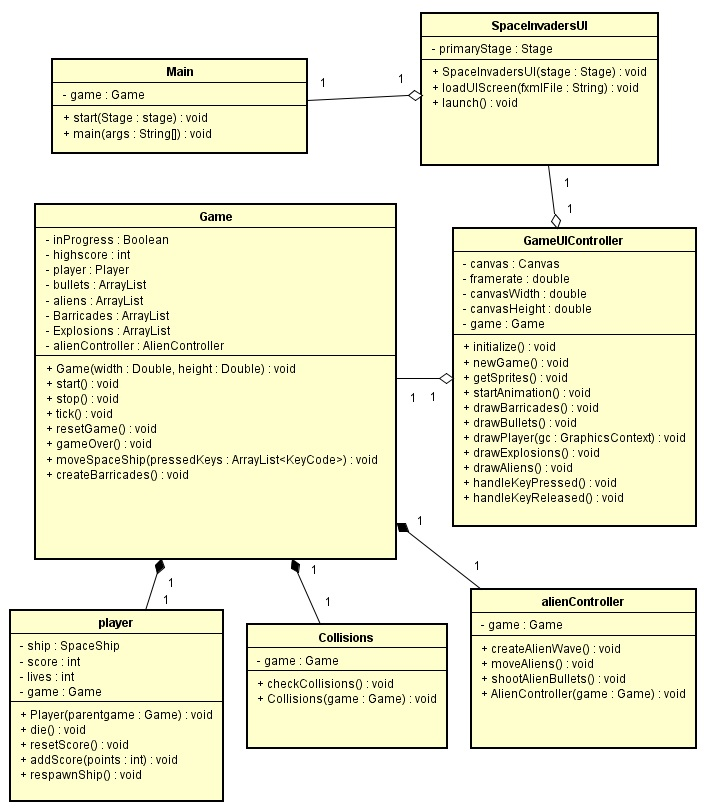
\includegraphics[width=14cm, height=16cm]{UMLSEM.jpg}
\caption{Main classes UML Class Diagram}
\end{figure}
\pagebreak

 \subsection*{Exercise 1.5} 
\begin{figure}[ht!]
\centering
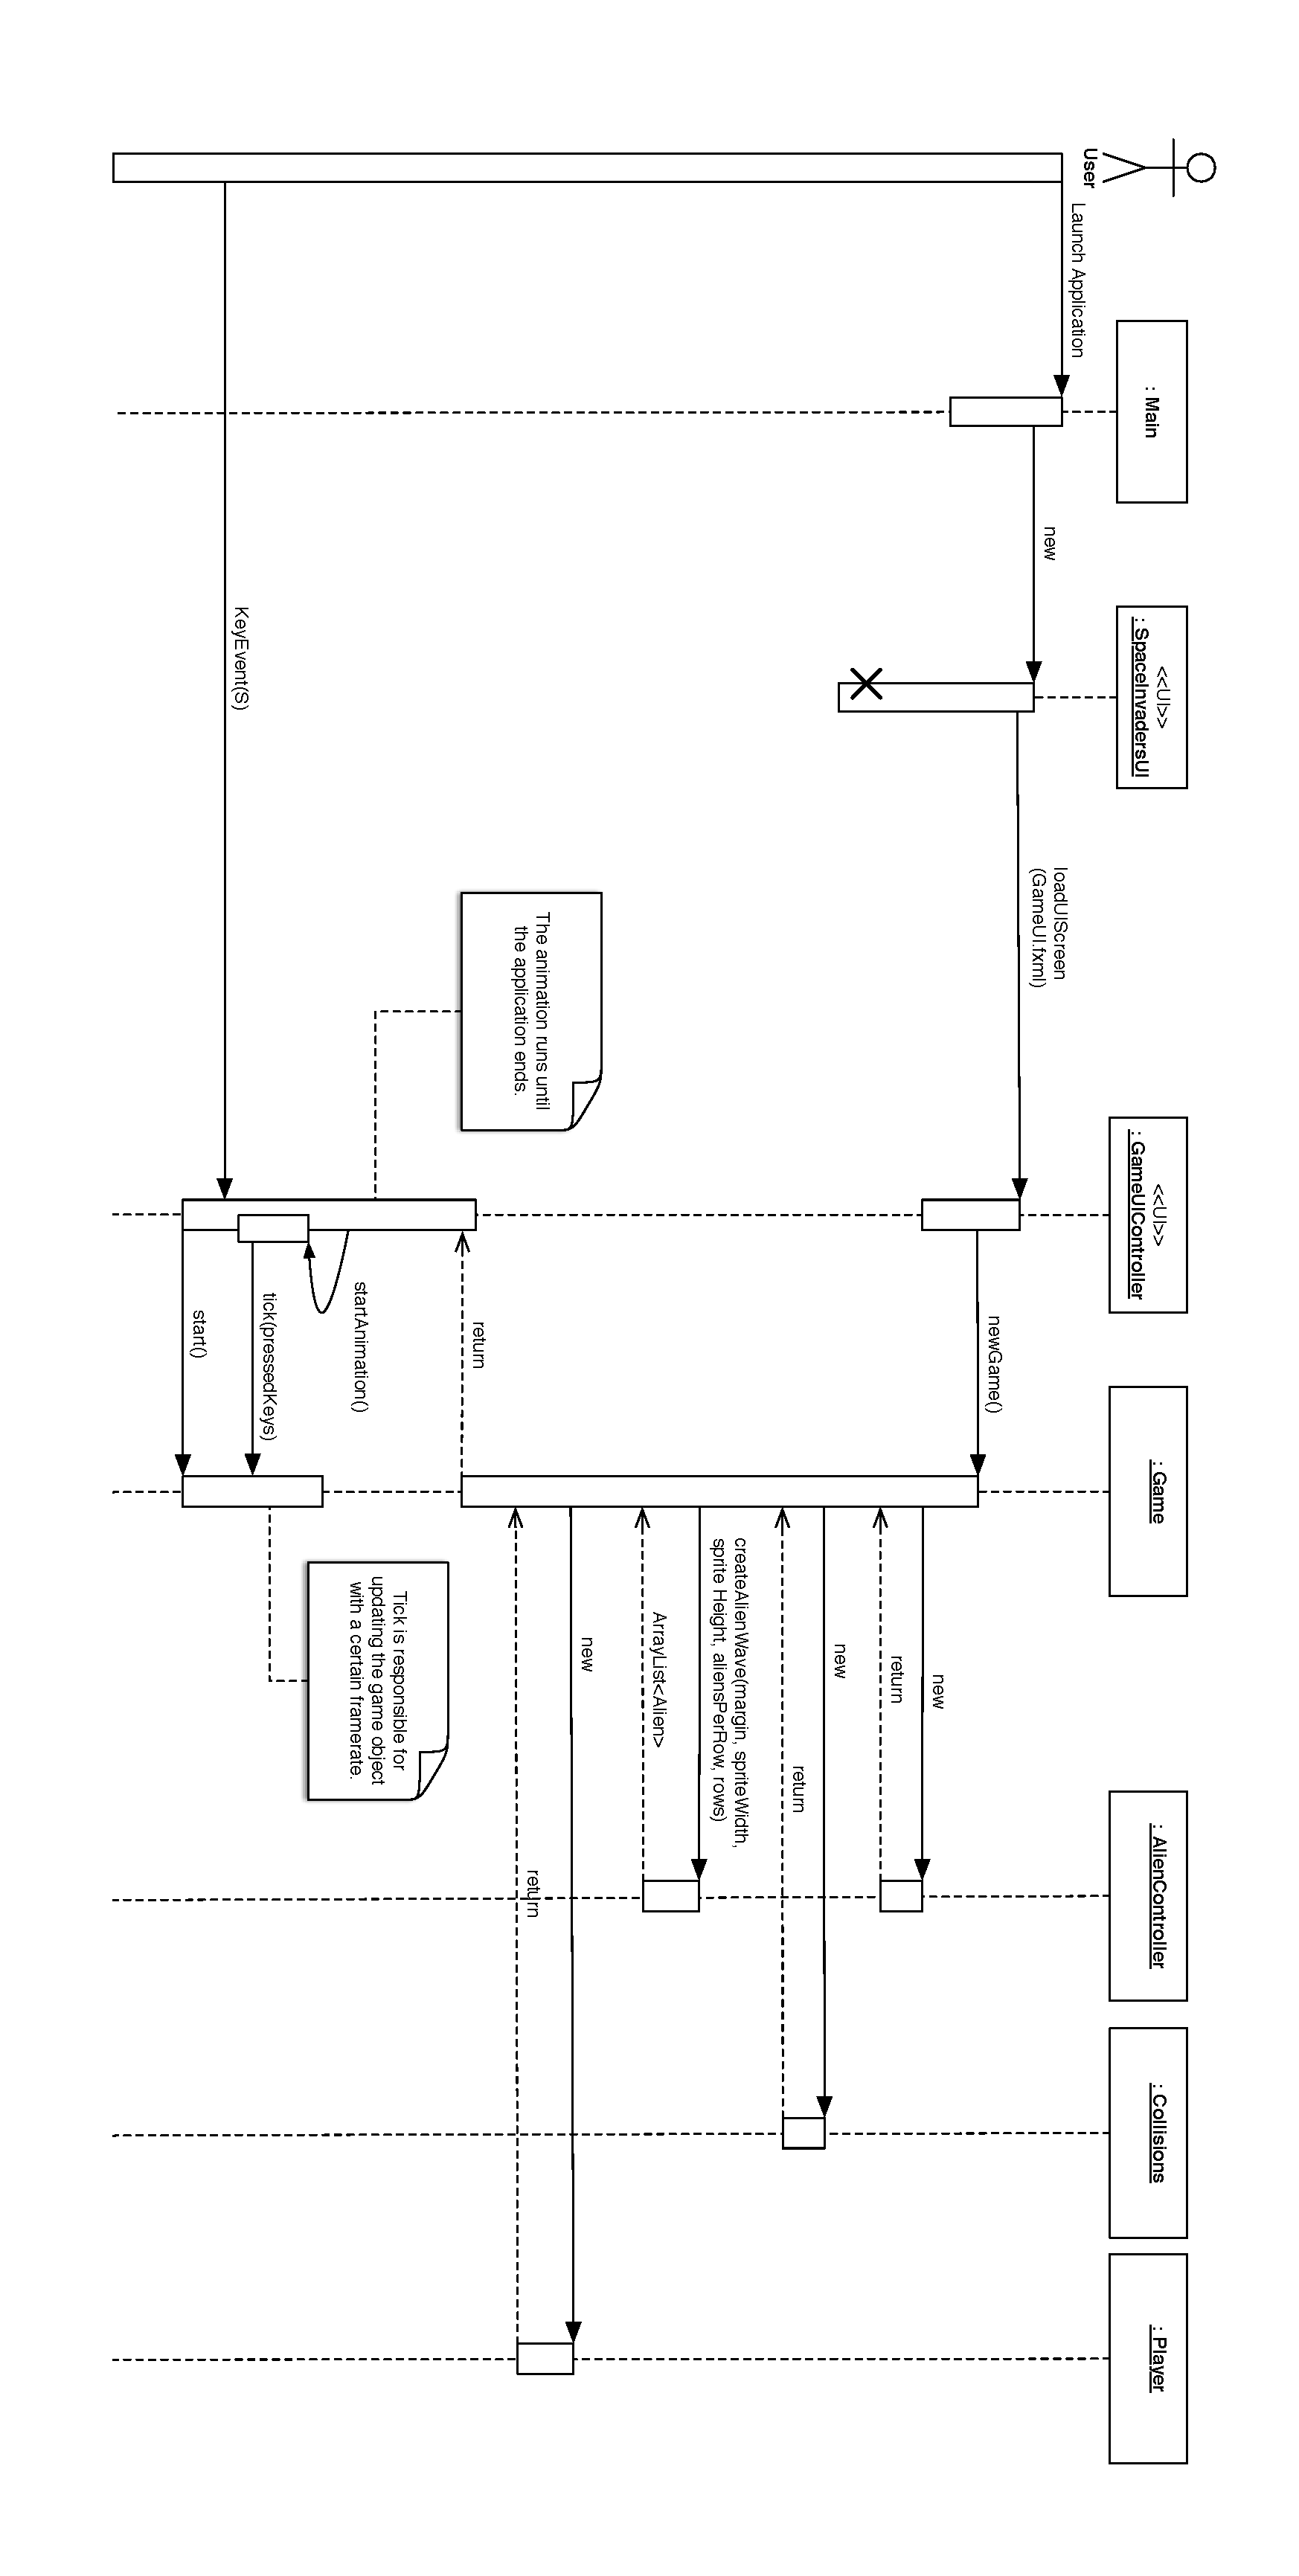
\includegraphics[width=0.6\textwidth]{SI-Sequence.pdf}
\caption{Main classes UML Sequence Diagram}
\end{figure}
This diagram contains the scenario of launching the game, until the player presses S to start the game.
\pagebreak

\section{Exercise 2 - UML in practice}
\subsection*{Exercise 2.1}
UML Aggregation applies to a "Consists of" relation.
Parts of the whole may be shared, which means that child classes can exist independent of the parent class.
If the parent is destroyed, the child can remain without the parent.

UML Composition applies to a "Contains" relation.
A part belongs to a whole. If the parent class does not exist, the child cannot exist separate of the parent. 
If the parent is destroyed, the child will also be destroyed.

Aggregation is used in the relations between the Game class and classes which assist the Game class.
A Game consists of multiple Units (players, aliens, barricades, explosions and bullets), Collisions and the alienController. These are a composition relation, because without these classes, it is not possible to play the game, thus making the Game class useless.

\subsection*{Exercise  2.2}
Parameterized, generic classes use type parameters which enable the user to re-use code for a different object type. 

An example of a parametrized class used in the project is the java.util.ArrayList class.
It takes an input Type, and allows creation of a list, reusing the same code for every object type.

The project itself does not contain classes using Parameterized classes.
\pagebreak
\subsection*{Exercise  2.3}
The project contains one major hierarchy, treating the different game Units. 
Within the hierarchy there is a sub-hierarchy for bullets. There are two bullet types, one for aliens and one for the player.
The subclasses directly linked to Unit are "Polymorphism" relations, since the behavior of each unit is different.
The subclasses of Bullet are "Is-A" relations, since they have the same behavior as their superclass.

\begin{figure}[ht!]
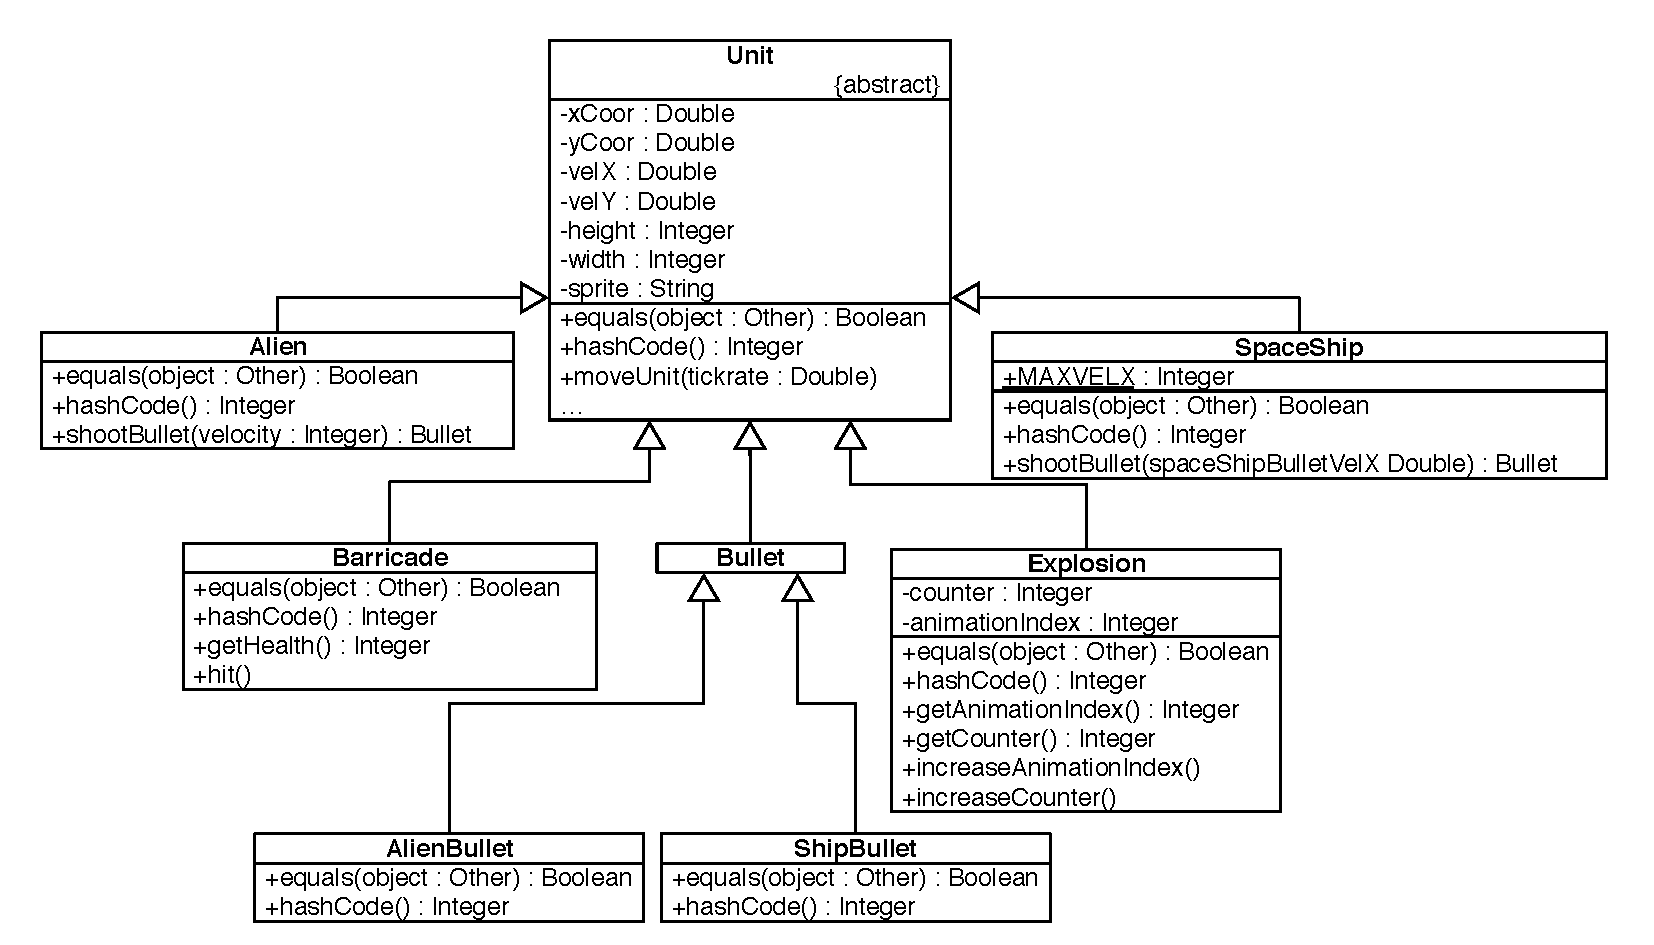
\includegraphics[width=1.1\textwidth]{SI-UMLhierarchies.pdf}
\caption{Unit hierarchy UML Class Diagram}
\end{figure}

\pagebreak
\section*{Excercise 3 - Simple Logging}
\subsection*{Exercise 3.1}

Responsibility driven design was used as a tool to develop the logger.
Starting with the requirements the following classes could be added to the product:

\begin{itemize}
\item Logger
\item LogPlayer
\item LogAliens
\item LogBullets
\item LogBarricades
\item LogExplosions
\item LogExceptions
\item LogErrors
\item WriteLog
\item ReadLog
\end{itemize}

Next the classes to be used were selected from the list. The following classes will be used:
\begin{itemize}
\item Logger
\item WriteLog
\end{itemize}

These classes were added to a table, listing their responsibilities:
\begin{center}
   \hspace*{-0.75in}\begin{tabular}{ | p{3cm} | p{5cm} | p{3cm} | p{2cm} | p{2cm} |}
  \hline
  Class & Responsibility & Collaborates with & Super & Sub \\ \hline
  Logger & Log all the actions in the game & WriteLog & & \\ \hline
  WriteLog & Write the log to a file & Logger & & \\ \hline
    \end{tabular}
\end{center}

\begin{figure}[ht!]
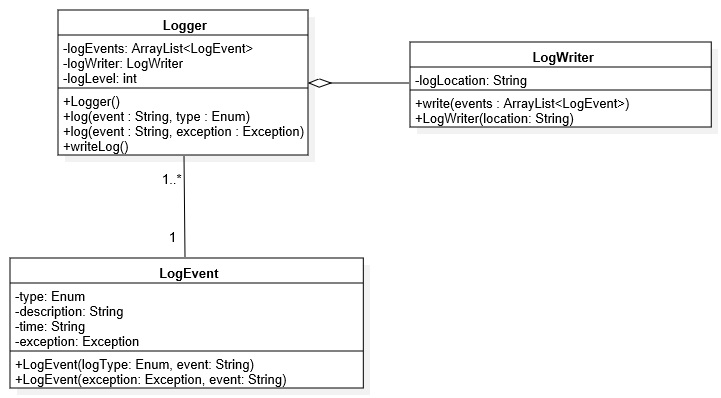
\includegraphics[width=1.1\textwidth]{LoggerUML.jpg}
\caption{Logger UML Class Diagram}
\end{figure}
\newpage

 \clearpage
\section*{Logger Functional Requirements}

A list of functional requirements considered for the extension of the game with a logger using the MoSCoW method described in the previous section.

\subsection*{Must Haves}
The Logger of the game must meet the following requirements:
\begin{itemize}
	\item The game shall be able to log all actions happening during execution the game.
	\item The logger shall be able to write the log to a file.
\end{itemize}

\subsection*{Should Haves}
The Logger of the game  should meet the following requirements:
\begin{itemize}
	\item The logger shall keep track of the time each action is executed.
	\item The logger shall have different logging levels.
	\item The logger shall be able to log exceptions thrown.
	\item The logger shall be able to log errors.
\end{itemize}

\subsection*{Could Haves}
The Logger of the game could meet the following requirements:
\begin{itemize}
	\item ...
\end{itemize}

\subsection*{Would/Won't Haves}
The Logger of the game won't meet the following requirements:
\begin{itemize}
	\item The logger shall use text colors in the output log.
\end{itemize}

\end{document}

